\newpage


\section{Prototyping}\label{sec:prototyping}

\subsection{Functional Selection}\label{subsec:functional-selection}

\subsubsection{Identifying Core Functionalities Based on User Needs}

In the functional selection phase, several key features were identified and extracted from the requirements gathered
during the Requirements Engineering process in \ref{sec:requirements-engineering}. These features were chosen based on
their potential to validate the core interaction and functionality of the chatbot system, ensuring that the prototype
effectively addresses the primary needs of the stakeholders. The focus was placed on fundamental aspects that would
provide a meaningful demonstration of the system’s capabilities without requiring full-scale implementation of the
entire product.

The first selected feature was the basic chat functionality, which forms the core of the user interaction with the
system. This functionality allows users to communicate their needs through a conversational interface, enabling the
chatbot to capture and process input in real-time. Given that the chatbot is designed to guide users through the process
of finding products and services, this feature is essential for testing how well the system can interpret user queries.

Secondly, the prototype incorporates a chat history feature, which ensures that users can review their previous
interactions with the chatbot. This functionality not only improves the user experience by providing continuity but also
allows for finishing started orders or asking questions to placed orders, enhancing the overall usability of the system.

A crucial element of the system is information extraction from the conversation, where the chatbot analyzes the user’s
input to identify specific needs. This feature is pivotal to understanding the customer's requirements, whether for
hardware, software, or services, and plays a central role in shaping the subsequent actions of the system.

The fourth selected feature is the matching of the extracted customer need with the supplier catalog. This functionality
ensures that the system can search the internal catalogs and identify the most relevant products or services that meet
the user's needs. This aspect of the prototype will demonstrate the effectiveness of the backend logic in delivering
accurate and relevant results from the catalog, allowing users to make informed decisions.

Lastly, order tracking was included as a feature to allow users to monitor the status of their requests after placing an
order. While not fully implemented in the prototype, this functionality simulates the experience of tracking an order's
progress, which is a vital part of the user journey in the final system.

By focusing on these selected features, the prototype can provide a realistic representation of how the final system
will handle key user interactions, offering valuable insights into both technical feasibility and user experience. The
selected features are not only aligned with stakeholder requirements but also serve as a solid foundation for evaluating
the prototype’s effectiveness in fulfilling the system's objectives.

\subsubsection{Breaking Down Core Functionalities into Specific Features}

After identifying the core functionalities that the system needs to fulfill, the next step is to break these down into
more specific features. Each of the basic functionalities, such as chat interaction, information extraction, and order
tracking, can be addressed with a combination of technical components and architectural decisions. By doing so, we
ensure that the prototype meets the user needs effectively while laying the groundwork for future development.

The first basic functionality, enabling chat interaction, requires more than just a user interface where users can type
messages. For this interaction to be meaningful, there must be a way to manage the exchange of information between the
frontend (where the user interacts) and the backend (where the logic and data processing occur). To achieve this, the
system should implement a RestAPI, which will allow seamless communication between the chatbot interface and the backend
services. This ensures that user inputs are received and processed efficiently, and responses are sent back in real-time
, creating a dynamic and responsive user experience. The RestAPI will act as the backbone for handling asynchronous
requests, ensuring that the system remains scalable and flexible as more complex features are added.

For the chat history feature, the system needs to ensure that users can retrieve past conversations, allowing them to
continue where they left off. This is essential for maintaining continuity, especially in scenarios where a user might
need to revisit an earlier request or clarify an ongoing conversation. To address this need, a PostgreSQL database
should be used. PostgreSQL is well-suited for this task due to its ability to handle structured data and complex queries
, ensuring that chat history can be stored and accessed efficiently. This database solution not only supports the
retrieval of individual conversations but also allows the system to manage user sessions, ensuring that each user can
securely access their personal chat history.

The ability to extract information from the conversation is another key feature that requires a more granular approach.
The chatbot needs to understand the specific needs expressed by the user—for example whether they are looking for
hardware, software, or services. This requires an intelligent system capable of processing natural language and
extracting relevant information. To accomplish this, the system should utilize \ac{GenAI}, which will be integrated
through an OpenAPI model. By leveraging \ac{AI}, the chatbot will be able to perform more advanced tasks, such as
recognizing the user’s intent, identifying key terms, and extracting actionable information from the conversation. This
goes beyond simple keyword matching, allowing the system to offer personalized and accurate results based on the user's
expressed needs.

Next, the system must provide users with the ability to retrieve their assigned chats after logging in. This need arises
from the requirement for users to be able to access their ongoing conversations from different devices or after a
session ends. To meet this need, a login page should be implemented where users can authenticate themselves and load
their assigned chats from the database. Upon successful login, the system should query the PostgreSQL database to
retrieve the user’s active or previous conversations, allowing for seamless continuation of their interactions with the
chatbot. This feature ensures that conversations are not lost and users can interact with the system across multiple
sessions. However, this feature should only be simulated in the prototype, as there will be a \ac{SSO} in the future,
but this may not be integrated without an internal Group \ac{PSA}.

In addition to these user-facing functionalities, the system must remember user settings, such as login states and
preferences, to provide a seamless experience. For example, users might choose between dark and light modes or prefer
not to re-enter their login credentials after refreshing the page. To ensure these preferences are maintained, the
system should utilize cookies. Cookies allow the system to store small pieces of information about the user’s
preferences and login state, ensuring that these settings are remembered across different sessions without requiring the
user to input them repeatedly.

Finally, beyond simple chat interactions, there is a need for the system to handle more complex user inputs, such as
file uploads. Users might need to upload documents—such as service descriptions—so the system can extract relevant
information. This requires the system to not only process unstructured text but also to extract actionable data from
uploaded files. To address this need, a file upload functionality should be integrated into the system. This feature
will allow users to upload documents, and the system, through OpenAIs model, can analyze the content and extract the
necessary information, such as service descriptions or specifications. This expands the chatbot’s functionality beyond
simple text interactions, allowing it to handle more complex user requirements and data inputs. %TODO Wurde das am Ende wirklich umgesetzt oder nur simuliert?

By breaking down these core functionalities into specific technical solutions, the prototype will be able to address the
key user needs effectively. The proposed technical features—such as the RestAPI for communication—ensure that the system
is both flexible and robust enough to meet its intended purpose. Each feature plays a crucial role in creating a
responsive, intelligent, and user-friendly system that will serve as a foundation for the final product.

\subsection{Construction}\label{subsec:construction}

\subsubsection{Frontend}

\paragraph{Project Setup}%

Main Application Entry Point

Vite Configuration

\paragraph{Project Folder Structure}

\paragraph{API Handling}

The \ac{API} handling is an essential part of the chatbot system, providing interaction between the frontend and the
backend. The \ac{API} connects various services, such as case management, message sending, and supplier handling, to
ensure that the system operates seamlessly. This section covers on one side the most important functions from the
\texttt{api.ts}, \texttt{v1.json}, and \texttt{v1.d.ts} files, which define the \ac{API}'s structure, types, and
requests. On the other side, there are three composables in the project that play a significant role in facilitating
\ac{API} interactions: \texttt{useApiClient.ts}, \texttt{useCasesApi.ts}, and \texttt{useMessagesApi.ts}. These
composables encapsulate \ac{API}-related logic, making it easier to reuse and manage the interactions between the
frontend and the backend.

The \texttt{api.ts}
file defines core types and utilities that are crucial for \ac{API} interactions. It leverages TypeScript's type system
to define \ac{API} schema models, ensuring that all requests and responses are strongly typed and consistent throughout
the application.

The following snippet defines the types for \texttt{Case}, \texttt{State}, and \texttt{Message}, as shown in Code
\ref{lst:api-core-types}.

% @formatter:off
\begin{lstlisting}[language=JavaScript, caption={Core API Types (\texttt{api.ts})},
  firstnumber=1,label={lst:api-core-types}]
export type Case = components['schemas']['Case']
export type State = ArrayType<NonNullable<components['schemas']['Case']['state']>>
export type Message = components['schemas']['Message'] & {
  loading?: boolean
}
\end{lstlisting}
% @formatter:on

The \texttt{Case}, \texttt{State}, and \texttt{Message} types are derived from the OpenAPI schema (defined in the
\texttt{v1.json} file). These types ensure that every interaction with the \ac{API} adheres to the structure
defined by the backend. The \texttt{Message} type is extended to include a \texttt{loading} property
, allowing the frontend to track when a message is being processed, providing better feedback to the user.

The \texttt{v1.json} file represents the OpenAPI schema forthe backend. It defines all available \ac{API} endpoints,
their parameters, and their expected responses. This structure is crucial for understanding how the frontend interacts
with the backend.

Code \ref{lst:api-v1-json}, stored in \ref{subsec:frontend}, defines the \texttt{/api/v1/cases} endpoint for listing and
creating cases.

This endpoint supports both listing (GET) and creating (POST) cases. The GET method allows
filtering by \texttt{user\_id} and limiting the number of cases retrieved. The POST method requires a
\texttt{CreateCaseRequest} body to create a new case.
Each operation has a unique \texttt{operationId} (e.g., \texttt{list\_cases\_api\_v1\_cases\_get}), which is
used to reference and document the \ac{API} call.

Because OpenAPI is used, the \ac{API} Endpoints can be shown in the schema from Swagger as shown in Figure
\ref{fig:swaggerui}.

\begin{figure}[H]
\centering
\caption[Swagger UI]{Swagger UI \footnotemark}
\label{fig:swaggerui}
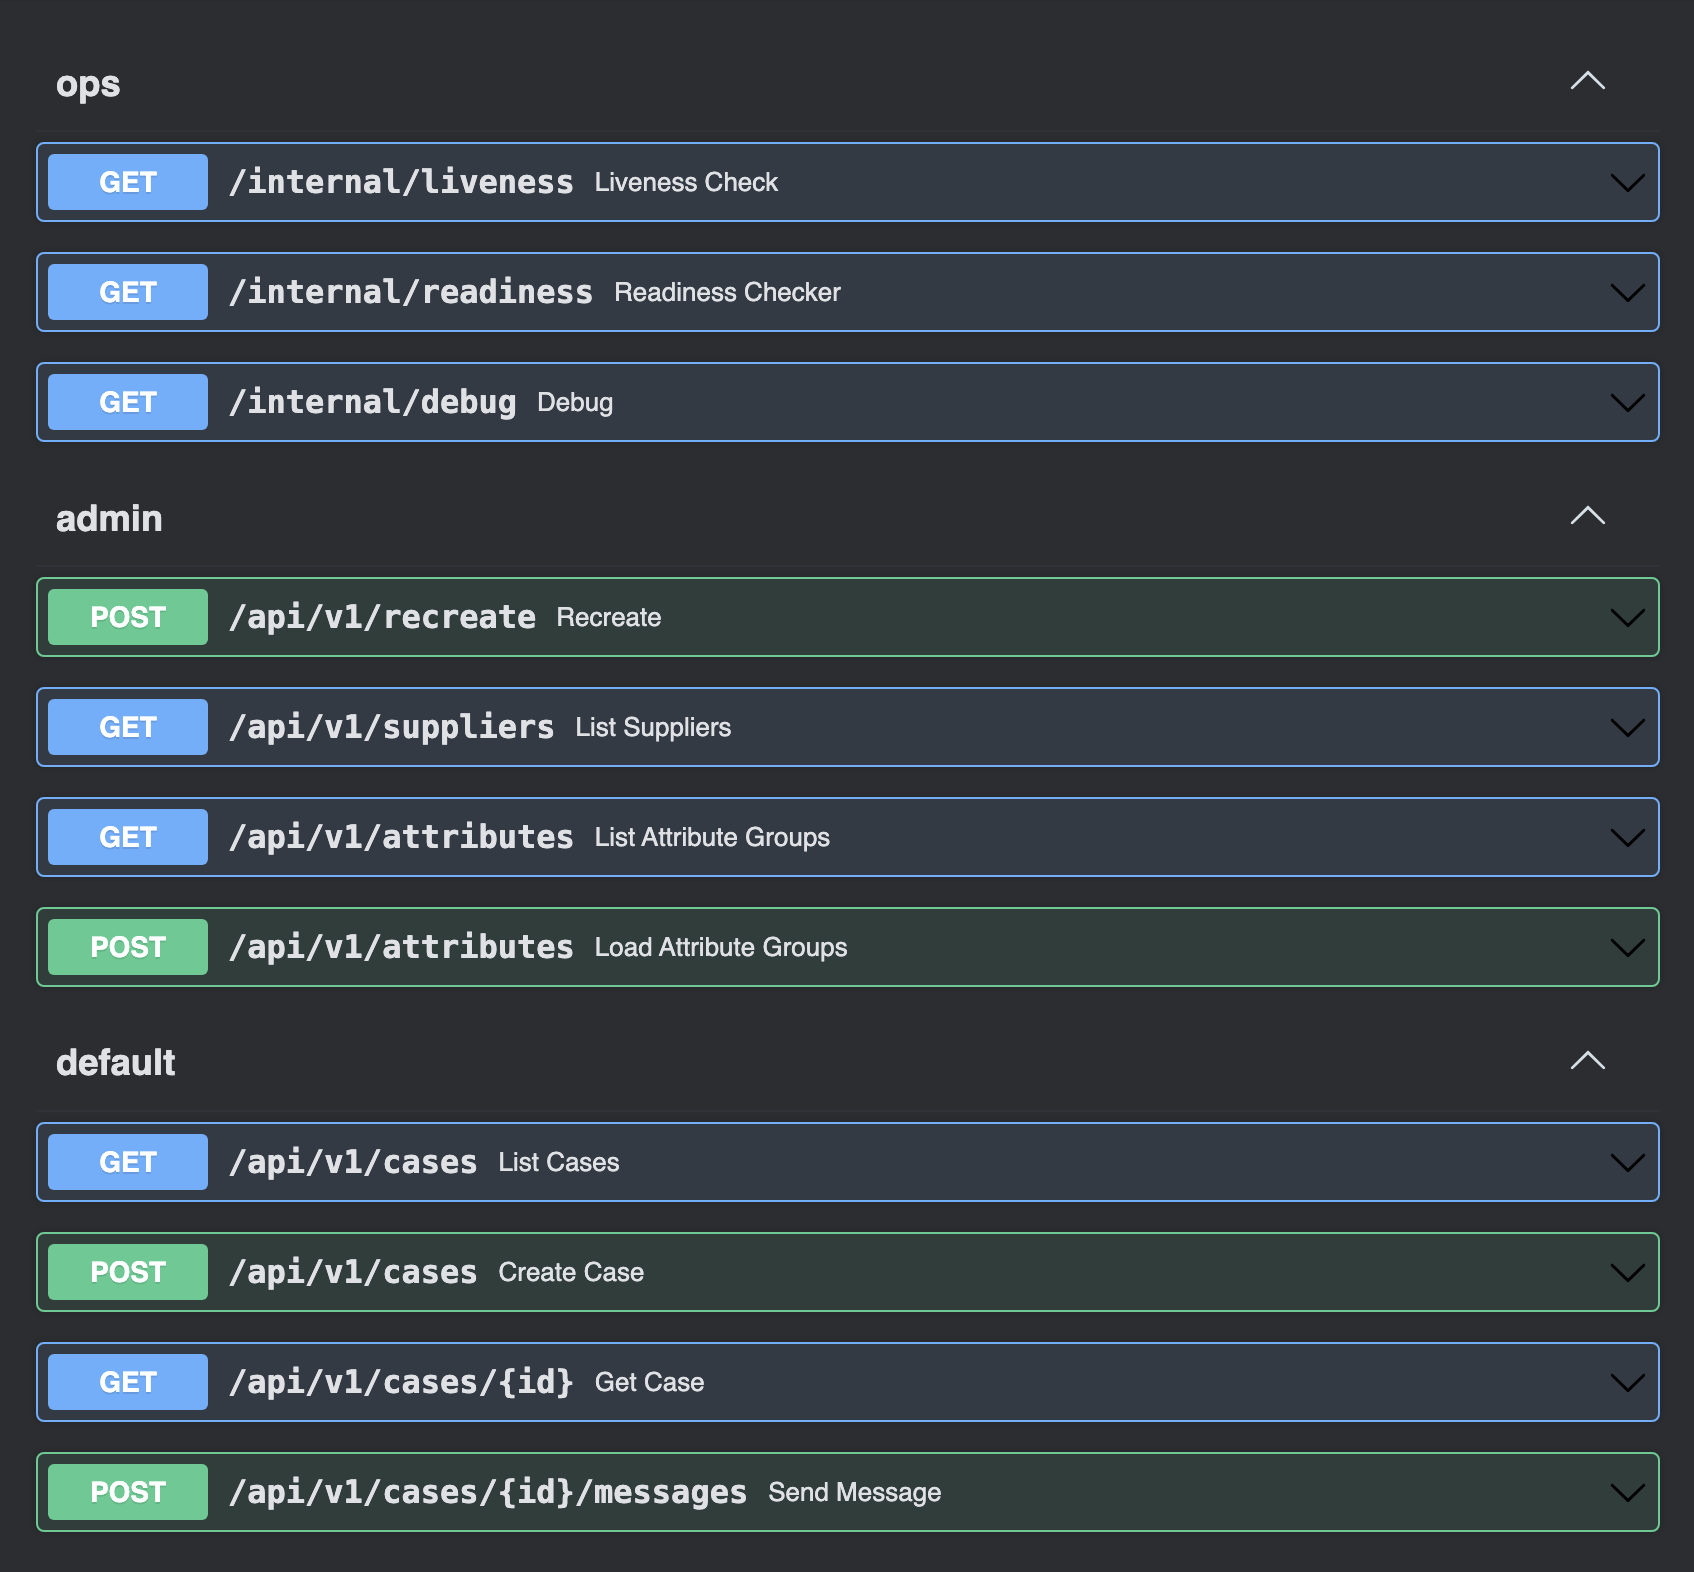
\includegraphics[width=1\textwidth]{abbildungen/Prototyping/Swagger_UI.png}
\end{figure}
\footnotetext{Own illustration}

This made it easy to test the \ac{API} Endpoints without implementing them directly in the code.

The \texttt{v1.d.ts} file defines the TypeScript types generated from
the OpenAPI schema, ensuring that all \ac{API} requests and
responses are typed correctly. This provides strong typing for all
interactions with the \ac{API}, helping prevent runtime errors and ensuring that the frontend and backend stay in sync.

The following snippet shows the type definition for the \texttt{Case} schema, as demonstrated in Code
\ref{lst:case-schema}.

% @formatter:off
\begin{lstlisting}[language=JavaScript, caption={Case Schema Definition (\texttt{v1.d.ts})},
  firstnumber=260,label={lst:case-schema}]
export interface components {
  schemas: {
    Case: {
      /**
      * Id
      * Format: uuid
      */
      id: string;
      /** State */
      state?: components["schemas"]["StateAttributeGroup"][];
      /** Messages */
      messages?: components["schemas"]["Message"][];
      /**
      * Created At
      * Format: date-time
      */
      created_at: string;
      /** Title */
      title?: string | null;
      case_type?: components["schemas"]["SystemCaseTypeEnum"] | null;
    };
  }
}
\end{lstlisting}
% @formatter:on

This schema defines the structure of a \texttt{Case} object, which includes fields such as \texttt{id
}, \texttt{state}, \texttt{messages}, \texttt{created\_at}, and optional fields like \texttt{title} and \texttt{
case\_type}. The \texttt{state} field contains an array of \texttt{StateAttributeGroup} objects
, while the \texttt{messages} field contains an array of \texttt{Message} objects, demonstrating the
complexity of the data model.

The \texttt{useApiClient.ts} file defines a function that sets up and returns an \ac{API} client. It uses the
\texttt{openapi-fetch} library to create a client that
interacts with the defined OpenAPI schema. The client is configured with a base URL, and headers can be added
as needed. This client serves as the primary way to make \ac{API} calls throughout the application.

Code \ref{lst:use-api-client} demonstrates how the \texttt{useApiClient} function is defined.

% @formatter:off
\begin{lstlisting}[language=JavaScript, caption={Setting up the API Client (\texttt{useApiClient.ts})},
  firstnumber=4,label={lst:use-api-client}]
export const useApiClient = () => {
  return createClient<paths>({
    baseUrl: import.meta.env.VITE_API_BASE_URL,
    headers: {
      // Authorization: `Basic ${import.meta.env.VITE_API_CREDENTIALS}`
    }
  })
}
\end{lstlisting}
% @formatter:on

The \texttt{useApiClient} function encapsulates
the configuration of the \ac{API} client, allowing other composables to easily import and use it. This approach keeps
the \ac{API} setup centralized and manageable, making it easy to configure base URLs and headers in one place.

The \texttt{useCasesApi.ts} file defines the composable for interacting with
cases-related \ac{API} endpoints. It utilizes the \ac{API} client to fetch and create cases and employs
\texttt{vue-query} for managing data caching, mutation, and state.

The following snippet shows how the \texttt{findAll} function is implemented using \texttt{vue-query}, as demonstrated
in Code \ref{lst:use-cases-api-findall}.

% @formatter:off
\begin{lstlisting}[language=JavaScript, caption={Fetching All Cases (\texttt{useCasesApi.ts})},
  firstnumber=19,label={lst:use-cases-api-findall}]
const findAll = useQuery({
  queryKey: ['cases'],
  queryFn: async () => {
    return (
      await client.GET('/api/v1/cases', {
        params: {
          query: {
            user_id: userStore.userId
          }
        }
      })
    ).data?.cases
  },
  ...defaultQueryOptions
})
\end{lstlisting}
% @formatter:on

This function uses \texttt{vue-query} to fetch all cases for a specific user.
It defines a \texttt{useQuery} with a unique \texttt{queryKey} (\texttt{['cases']}) and a \texttt{queryFn} that performs
a GET request to the \texttt{/api/v1/cases} endpoint, passing the user's ID as a query parameter. The
default options are applied to the query to manage retry behavior and error handling.

The \texttt{useCasesApi} composable also includes functions for creating a case and fetching a
case by its ID. It leverages Vue's reactivity to make
these operations seamless within the application, allowing components to respond automatically to changes in the data.

The \texttt{useMessagesApi.ts} file defines the composable for interacting with message-related
\ac{API} endpoints. It primarily handles sending messages for a given
case and fetching the list of messages. Similar to \texttt{useCasesApi.ts}, this composable uses the shared \texttt
{useApiClient} and integrates with \texttt{vue-query} for data management.

The \texttt{create} function in \texttt{useMessagesApi} sends a new message to the
backend by making a POST request to \texttt{/api/v1/cases/\{id\}/messages}, with the message content
as the request body. This function allows the chatbot to send user-generated messages and system messages effectively.

The composable \texttt{useMessagesApi.ts} also includes a \texttt{findAll} function to fetch all
messages associated with a specific case. This function is accomplished
by extending the \texttt{findById} method from \texttt{useCasesApi}, ensuring consistency in handling \ac{API}
interactions across the project.


\paragraph{User Login and Session Handling}%UserLoginDialog.vue

This section focuses on the user login and session management, enabling users to authenticate themselves by entering a
User \ac{ID}. The system leverages Vue.js components, Vuetify elements, and reactive state management to build an
intuitive login dialog. This feature ensures that only authenticated users can interact with the chatbot, thus
personalizing the user experience and maintaining the session across multiple interactions.

The login component is implemented using \ac{TS}, providing type safety and enhanced tooling support, which is
beneficial for large-scale projects. Below is a breakdown of the code's key functionalities.

The following code snippet imports essential modules and components used throughout the login process. See
Code \ref{lst:importing-dependencies}.

\begin{lstlisting}[language=JavaScript, caption={Importing Dependencies (\texttt{UserLoginDialog.vue})},
firstnumber=2,label={lst:importing-dependencies}]
import { userStore } from '@/stores/user-store'
import { onUpdated, ref, useTemplateRef } from 'vue'
import { VTextField } from 'vuetify/components/VTextField'
\end{lstlisting}

The \texttt{userStore}
is imported from a centralized state management store to handle user-specific data, such as the user \acs{ID}. The
\texttt{onUpdated}, \texttt{ref}, and \texttt{useTemplateRef} functions are imported from Vue, essential for reactive
programming, where component properties update automatically when the state changes. The \texttt{VTextField} from
Vuetify is used to render the input field in the login form.

Reactive references and validation rules are established in Code \ref{lst:reactive-variables-validation} to handle user
input.

\begin{lstlisting}[language=JavaScript, caption={Reactive Variables and Validation (\texttt{UserLoginDialog.vue})},
firstnumber=6,label={lst:reactive-variables-validation}]
const model = defineModel<boolean>()
defineProps<{ persistend: boolean }>()

const userIdInput = useTemplateRef<VTextField>('userIdInput')
const userId = ref<string>()
const userIdRules = ref<((v: string) => string | boolean)[]>([
(v: string) => (!!v && !!v.trim()) || 'User ID is required'
])
\end{lstlisting}

The \texttt{model} defines a reactive model to control the visibility of the login dialog, while the \texttt{persistend}
prop determines whether the dialog can be closed without user interaction. The \texttt{userId}
is a reactive reference holding the user input, while \texttt{userIdRules}
ensures that the input is valid, requiring a non-empty string to maintain data integrity.

The \texttt{onUpdated} lifecycle hook, shown in Code \ref{lst:synchronizing-lifecycle-hooks}, ensures the synchronization
of the user \acs{ID} with the session state stored in the \texttt{userStore}.

\begin{lstlisting}[language=JavaScript, caption={Synchronizing State with Lifecycle Hooks (\texttt{UserLoginDialog.vue})},
firstnumber=15,label={lst:synchronizing-lifecycle-hooks}]
onUpdated(() => {
userId.value = userStore.userId
})
\end{lstlisting}

This ensures that the correct user \acs{ID} is displayed in the form if it has been previously set.

Code \ref{lst:handling-user-login} handles the user login process.

\begin{lstlisting}[language=JavaScript, caption={Handling User Login (\texttt{UserLoginDialog.vue})},
firstnumber=19,label={lst:handling-user-login}]
function login() {
if (!userId.value) return

userStore.login(userId.value)
model.value = false
}
\end{lstlisting}

The \texttt{login} function first checks if the \texttt{userId} field is populated. If so, the
\texttt{userStore.login()} function is called to store the user \acs{ID} for future interactions. After a successful login,
the login dialog is closed, providing a seamless user experience.

The \ac{HTML} template uses Vuetify components to create the login interface, binding state variables for reactivity and
ensuring user input validation.

The login dialog is defined as follows in Code \ref{lst:login-dialog}.

\begin{lstlisting}[language=JavaScript, caption={Login Dialog (\texttt{UserLoginDialog.vue})},
firstnumber=28,label={lst:login-dialog}]
<v-dialog v-model="model" max-width="400" :persistent="persistend">
<template #activator="{ props: activatorProps }">
<v-btn v-bind="activatorProps" variant="text" class="text-none">
<div v-if="userStore.userId">{{ userStore.userId }}</div>
<div v-else>Login</div>
<template #append>
<v-icon v-if="userStore.userId">mdi-account-check</v-icon>
<v-icon v-else>mdi-account-plus</v-icon>
</template>
</v-btn>
</template>
</v-dialog>
\end{lstlisting}

The \texttt{v-model} directive links the dialog's visibility to the \texttt{model}
reactive variable. If the user is logged in (i.e., \texttt{userStore.userId}
is set), the button displays the user \acs{ID}; otherwise, it prompts the user to log in. Icons are dynamically displayed to
indicate the login state.

The input field for the user \acs{ID} is defined as shwon in Code \ref{lst:user-id-input}.

\begin{lstlisting}[language=JavaScript, caption={User ID Input Field (\texttt{UserLoginDialog.vue})},
firstnumber=57,label={lst:user-id-input}]
<v-text-field
ref="userIdInput"
v-model="userId"
:counter="10"
:rules="userIdRules"
label="User ID"
@keyup.enter="login"
clearable
></v-text-field>
\end{lstlisting}

The \texttt{v-text-field} is bound to the \texttt{userId} reactive reference, with a 10-character limit enforced by the
\texttt{counter} attribute. Validation rules are applied via \texttt{userIdRules}
, ensuring that users cannot submit invalid \acsp{ID}. The \texttt{@keyup.enter="login"}
directive enables users to press "Enter" to submit the form, simplifying interaction.

The login button is implemented as follows. See Code \ref{lst:login-button}.

\begin{lstlisting}[language=JavaScript, caption={Login Button (\texttt{UserLoginDialog.vue})},
firstnumber=70,label={lst:login-button}]
<v-btn @click="login" :disabled="!userId"> Login </v-btn>
\end{lstlisting}

The button is enabled only when a valid \texttt{userId}
is present, preventing users from submitting the form without valid input.

User login and session handling are critical for managing how users access the chatbot system. It ensures that only
authorized users can interact with the chatbot, which is essential for both security and personalization. Vuetify
components provide a professional and responsive interface, while Vue’s reactive system handles the dynamic nature of
login states, ensuring a smooth user experience without unnecessary page reloads or delays.

\paragraph{Storing Information}%folder stores

This section focuses on how the chatbot system stores and manages key pieces of data related to user sessions and
selected cases. Proper state management and persistence of information are crucial for maintaining a seamless user
experience, especially when handling interactions across multiple sessions or refreshing the application. Two key pieces
of state—the selected case and the user session—are managed using Vue's reactivity system. The state is stored locally,
allowing the application to maintain important information between page loads.

The \texttt{selected-case.store.ts}
file manages the state of the selected case throughout the chatbot session. It uses Vue's \texttt{reactive}
function to create a reactive store that can be shared across components. This is essential for keeping the selected
case in sync across different parts of the application.

The following code snippet shows how the \texttt{selectedCaseStore} is set up and managed, as demonstrated in
\ref{lst:selected-case-store}.

% @formatter:off
\begin{lstlisting}[language=JavaScript, caption={Setting up the Case Store (\texttt{selected-case.store.ts})},
  firstnumber=10,label={lst:selected-case-store}]
export const selectedCaseStore = reactive<CaseStore>({
  case: {
    id: '',
    created_at: ''
  },
  setCase(caseData: Case) {
    this.case = caseData
  },
  clearCase() {
    this.case = {
      id: '',
      created_at: ''
    }
  }
})
\end{lstlisting}
% @formatter:on

In this snippet, \texttt{selectedCaseStore}
is a reactive object that holds the current case state. This object provides essential methods to manage the state. The
\texttt{setCase}
method updates the case state with new data whenever a case is selected, ensuring that the correct data is displayed
across components when switching between different cases during a chat session. Additionally, the \texttt{clearCase}
method resets the case state, which is particularly useful when the user finishes working on a case or logs out.

By using a reactive store, the case state remains in sync across all components that rely on it, making the user
experience consistent and dynamic.

The \texttt{user-store.ts}
file handles the state of the user's session, including login and logout functionality. It uses Vue’s reactive system in
combination with the \texttt{useLocalStorage} utility from the \texttt{@vueuse/core} library to persist the user's
\texttt{userId} across sessions.

The following code snippet shows how the \texttt{userStore}
manages the user’s login and session data, as demonstrated in \ref{lst:user-store}.

% @formatter:off
\begin{lstlisting}[language=JavaScript, caption={Managing the User Session (\texttt{user-store.ts})},
  firstnumber=4,label={lst:user-store}]
const storedUserId = useLocalStorage<string | undefined>('user-id', undefined)

export const userStore: User = reactive<User>({
  userId: storedUserId.value,
  login(userId: string) {
    storedUserId.value = userId
    this.userId = userId
  },
  logout() {
    storedUserId.value = undefined
    this.userId = undefined
  }
})
\end{lstlisting}
% @formatter:on

This code leverages Vue’s reactive system in combination with the \texttt{useLocalStorage} utility from the
\texttt{@vueuse/core} library to ensure that the user’s
\texttt{userId} persists across sessions. The implementation begins
by initializing \texttt{storedUserId} from local storage, and this value is then used as the default for
\texttt{userId} within the reactive store.

When the \texttt{login} method is triggered, the user’s \texttt{userId} is stored both in the reactive
state and in local storage, allowing other components to reactively update based on the user’s login status. Conversely,
when the \texttt{logout} method is executed, both the reactive state and local storage are cleared,
ensuring that the session is properly ended when the user logs out.

This approach ensures that the user does not have to log in again after refreshing the page or
closing and reopening the application, thanks to the persistence of the \texttt{userId} in local storage.


\paragraph{Basic Chat Functionality}%Chat.vue, ChatInput.vue, ChatMessage.vue

The basic chat functionality enables users to interact with the chatbot, allowing both text-based communication and
document uploads. This functionality is powered by five components: \textit{Chat.vue}
for managing the chat interface, \textit{ChatInput.vue} for handling user input, \textit{ChatMessage.vue} for rendering
individual messages, \textit{ChatHistory.vue} for rendering the conversation and \textit{MessageLoadingAnimation.vue}
for the loading animation. Each of these components is explained in detail below.

The \texttt{Chat.vue}
component is responsible for managing user interactions with the chatbot, including sending messages and uploading
files. It communicates with the backend via API calls and dynamically updates the chat history as messages are sent and
received. The structure incorporates composables for fetching data and managing state, as well as improved handling of
file selection.

The following code snippet demonstrates the updated imports and setup for the component, which includes composables for
managing API interactions and a reactive store for handling the selected case. This is shown in
Code \ref{lst:chat-updated-imports}.

% @formatter:off
\begin{lstlisting}[language=JavaScript, caption={Updated Imports and Setup (\texttt{Chat.vue})},
  firstnumber=2,label={lst:chat-updated-imports}]
import { useCasesApi } from '@/composables/useCasesApi'
import { useMessagesApi } from '@/composables/useMessagesApi'
import { selectedCaseStore } from '@/stores/selected-case.store'
import { Message } from '@/types/api'
import _ from 'lodash'
import { computed, ref, useTemplateRef } from 'vue'
\end{lstlisting}
% @formatter:on

In this snippet, \texttt{useCasesApi} and \texttt{useMessagesApi} are custom composables that
handle API calls for retrieving and managing case data and
messages. The \texttt{selectedCaseStore} stores the currently selected
case, ensuring that messages are linked to the correct context.

Several reactive variables are defined to track the state of the message being sent and the system’s response, as shown
in Code \ref{lst:chat-reactive-variables}.

% @formatter:off
\begin{lstlisting}[language=JavaScript, caption={Reactive Variables for Message Tracking (\texttt{Chat.vue})},
  firstnumber=10,label={lst:chat-reactive-variables}]
const pendingMessage = ref<Message | undefined>()
const responseLoadingMessage = ref<Message | undefined>()

const messagesApi = useMessagesApi(selectedCaseId)
const casesApi = useCasesApi()
\end{lstlisting}
% @formatter:on

The \texttt{pendingMessage} holds the message
that the user is sending, while \texttt{responseLoadingMessage} tracks when the system is processing a response,
providing visual feedback to the user. These variables are essential
for enhancing the user experience by showing that the system is actively handling the request.

The \texttt{sendMessage} function sends the user’s message to the backend and handles the system’s response. The
function is detailed in Code \ref{lst:chat-send-message}.

% @formatter:off
\begin{lstlisting}[language=JavaScript, caption={Send Message Function (\texttt{Chat.vue})},
  firstnumber=32,label={lst:chat-send-message}]
const sendMessage = async (message: string) => {
  pendingMessage.value = {
    content: message,
    role: 'user',
    timestamp: new Date().toISOString()
  }

  responseLoadingMessage.value = {
    content: '',
    role: 'system',
    timestamp: new Date().toISOString(),
    loading: true
  }

  const result = await messagesApi.create.mutateAsync({
    content: message
  })

  if (result) {
    selectedCaseStore.case.state = result.state
    selectedCaseStore.case.messages = result.messages

    if (selectedCaseStore.case.title !== result.title) {
      selectedCaseStore.case.title = result.title
      casesApi.findAll.refetch()
    }
  }

  pendingMessage.value = undefined
  responseLoadingMessage.value = undefined
}
\end{lstlisting}
% @formatter:on

This function updates the local state to reflect that
a message is being sent and that the system is processing a response. The message is sent using \texttt{
messagesApi}, and once a response is received, the chat state is updated, and any visual indicators
(such as the loading message) are cleared. This ensures a smooth and responsive chat interface.

The template for \texttt{Chat.vue} renders the chat history via the \texttt{ChatHistory}
component and includes the message input field (\texttt{ChatInput}), as shown in Code \ref{lst:chat-template}.

% @formatter:off
\begin{lstlisting}[language=HTML, caption={Template for Chat.vue (\texttt{Chat.vue})},
  firstnumber=73,label={lst:chat-template}]
<template>
  <div v-if="selectedCaseId" class="bg-surface">
    <ChatHistory
      :messages="messages"
      :is-fetching="messagesApi.findAll.isFetching.value && false"
      @break-ice-with-message="sendMessage($event)"
      @break-ice-with-document="showFilePicker"
    />
    <ChatInput
      @send-message="sendMessage($event)"
      @show-file-picker="showFilePicker"
      @clear-file-selection="clearFileSelection"
      :selected-file-name="selectedFile?.name"
      :disabled="messagesApi.findAll.isFetching.value"
    />
    <input id="fileUpload" type="file" ref="fileUpload" @change="selectFile" hidden />
  </div>

  <span v-else class="d-flex flex-column h-100 justify-center" align-center ga-2 bg-surface">
    <v-icon class="opacity-50" color="blue-50" size="60" icon="$chat" />
    <b>Case required</b>
    <div class="text-center">To start communicating, create or select a case first.</div>
  </span>
</template>
\end{lstlisting}
% @formatter:on

The \texttt{ChatHistory} component is responsible for rendering the conversation, while \texttt{ChatInput} provides the
user with an input field to send messages. The template ensures that both messages and files can be sent and provides
feedback to the user while data is being fetched.

The component \texttt{ChatInput.vue} handles user input, including text messages and file uploads. It allows users to
compose messages and trigger specific actions like sending or attaching files.

The Code \ref{lst:define-msg-events} sets up the message input and prepares the component for emitting events when the
user sends a message or selects a file.

% @formatter:off
\begin{lstlisting}[language=JavaScript, caption={Defining Message and Emitting Events (\texttt{ChatInput.vue})},
firstnumber=4,label={lst:define-msg-events}]
const message = ref('')

const { selectedFileName = undefined } = defineProps<{ selectedFileName: string | undefined }>()
const emit = defineEmits<{
  sendMessage: [message: string]
  showFilePicker: []
  clearFileSelection: []
}>()
\end{lstlisting}
% @formatter:on

The \texttt{message} is a reactive reference that tracks the user’s input, and \texttt{selectedFileName}
tracks any file selected by the user. The \texttt{emit}
function enables communication with the parent component, notifying it when a message is sent or the file picker is
triggered. This ensures dynamic UI updates and seamless interactions.

The core function for sending messages is defined in Code \ref{lst:send-message-function}.

% @formatter:off
\begin{lstlisting}[language=JavaScript, caption={Send Message Function (\texttt{ChatInput.vue})},
firstnumber=13,label={lst:send-message-function}]
function sendMessage() {
  if (message.value) {
    emit('sendMessage', message.value)
    message.value = ''
  }
}
\end{lstlisting}
% @formatter:on

When the user presses "Enter" or clicks the send button, the \texttt{sendMessage} function emits the
\texttt{sendMessage} event and resets the input field. This provides smooth and intuitive message handling.

The message input field is set up with actions for sending messages and handling file uploads in the template of Code
\ref{lst:chatinput-template} and Code \ref{lst:trigger-buttons}.

% @formatter:off
\begin{lstlisting}[language=JavaScript, caption={Message Input Field (\texttt{ChatInput.vue})},
firstnumber=23,label={lst:chatinput-template}]
<v-text-field
  v-model="message"
  @keydown.enter.prevent="sendMessage"
  bg-color="surface"
  variant="outlined"
  color="primary"
  placeholder="Enter message..."
  rounded="lg"
  no-resize
  hide-details
>
\end{lstlisting}
% @formatter:on

% @formatter:off
\begin{lstlisting}[language=JavaScript, caption={Trigger Buttons (\texttt{ChatInput.vue})},
firstnumber=47,label={lst:trigger-buttons}]
<v-btn
  @click.prevent="emit('showFilePicker')"
  variant="text"
  size="small"
  density="default"
  icon="$paperclip"
  color="secondary"
/>
<v-divider vertical></v-divider>
<v-btn
  @click="sendMessage"
  :disabled="!message && !selectedFileName"
  variant="text"
  density="default"
  icon="$send"
  size="small"
  color="secondary"
/>
\end{lstlisting}
% @formatter:on

The \texttt{v-text-field} is bound to the reactive \texttt{message}
property, automatically reflecting user input. The attached buttons allow users to trigger the file picker or send a
message, ensuring the interface is user-friendly with easy-to-access actions.

The component \texttt{ChatMessage.vue} is responsible for rendering individual chat messages, differentiating between
messages sent by the user and those from the system or the chatbot. It also incorporates a loading animation for
messages still being processed.

The Code \ref{lst:chatmessage-props} shows how the props are defined and used in the component.

% @formatter:off
\begin{lstlisting}[language=JavaScript, caption={Defining Message Props (\texttt{ChatMessage.vue})},
firstnumber=2,label={lst:chatmessage-props}]
import { Message } from '@/types/api'

defineProps<Message>()
\end{lstlisting}
% @formatter:on

This component accepts a \texttt{Message} object as a prop, which contains details about the message content, its sender
, and its status.

Messages are displayed differently based on their role, as shown in the Code \ref{lst:message-display}.

% @formatter:off
\begin{lstlisting}[language=JavaScript, caption={Message Display Based on Role (\texttt{ChatMessage.vue})},
firstnumber=8,label={lst:message-display}]
<div
class="chat-message-row"
:class="{
  'justify-start': role === 'assistant' || role === 'system',
  'justify-end': role === 'user'
  }"
  >
  <div class="chat-message" :class="role">
    <div class="system-icon">
      <v-icon color="white" size="small" icon="$emojiHappy" />
    </div>

    <MessageLoadingAnimation v-if="loading" />
    <div v-else class="chat-message-text">{{ content }}</div>

    <div class="user-icon">
      <v-icon color="white" icon="mdi-account" />
    </div>
  </div>
</div>
\end{lstlisting}
% @formatter:on

Because of \texttt{<MessageLoadingAnimation v-if="loading" />} a loading animation is displayed if the message is still
loading; otherwise, the message content is shown. Messages are aligned based on their role, with user messages appearing
on the right and assistant or system messages on the left. This visual distinction helps users easily identify the
origin of each message, making the chat interface more intuitive.

The messages are styled based on the \texttt{role}, with specific colors and padding applied to distinguish between
different types of messages. See Code \ref{lst:message-style} for the styling of user messages.

% @formatter:off
\begin{lstlisting}[language=JavaScript, caption={Message Style Based on Role (\texttt{ChatMessage.vue})},
firstnumber=50,label={lst:message-style}]
&.user {
  align-items: flex-start;

  .system-icon {
    display: none;
  }

  .user-icon {
    display: block;
  }

  .chat-message-text {
    background-color: rgba(var(--v-theme-secondary), 0.1);
    margin-right: 12px;
    border-radius: 10px 0 10px 10px;
    padding: 8px 14px;
  }
}
\end{lstlisting}
% @formatter:on

The user messages are styled with a secondary theme color and appropriate padding to enhance readability and visually
separate them from messages originating from the assistant or system. This contributes to a clearer and more
aesthetically pleasing chat interface. Same is done with \texttt{&.system} or \texttt{&.assistant} with different
styling.

The \texttt{MessageLoadingAnimation.vue} component provides a simple, bouncing loader animation that is displayed
when the chatbot is processing a message. This component gives users feedback that the system is still working,
preventing confusion during response delays.

The following template renders the bouncing loader animation, which consists of three small dots that bounce in
a sequential animation. This behavior is shown in Code \ref{lst:bouncing-loader-template}.

% @formatter:off
\begin{lstlisting}[language=JavaScript, caption={Bouncing Loader Template (\texttt{MessageLoadingAnimation.vue})},
firstnumber=4,label={lst:bouncing-loader-template}]
<div class="bouncing-loader">
  <div></div>
  <div></div>
  <div></div>
</div>
\end{lstlisting}
% @formatter:on

This code creates the basic structure for the loader animation, where three div
elements are used to represent the dots that will bounce during the loading process.

The corresponding \ac{CSS} defines the animation behavior for the loader, creating a smooth, continuous bouncing effect.
The \ac{SCSS} code in Code \ref{lst:bouncing-loader-css} applies the necessary styling.

% @formatter:off
\begin{lstlisting}[language=JavaScript, caption={Bouncing Loader Animation (\texttt{MessageLoadingAnimation.vue})},
firstnumber=18,label={lst:bouncing-loader-css}]
.bouncing-loader > div {
  animation: bouncing-loader 0.6s infinite alternate;
}

@keyframes bouncing-loader {
  to {
    opacity: 0.1;
    transform: translate3d(0, -5px, 0);
  }
}
\end{lstlisting}
% @formatter:on

The \texttt{bouncing-loader} class assigns an animation to each dot. The keyframes define the
animation, where the opacity of the dots decreases to 0.1, and they move slightly upwards, creating the bouncing effect.

The \texttt{ChatHistory.vue} component is responsible for displaying the chat messages in a scrollable interface.
It uses Vuetify’s \texttt{v-virtual-scroll} to ensure efficient rendering, even with a large message history.

The Code  \ref{lst:chat-history-setup} shows the setup for this component, including reactive
data and the \texttt{scrollToBottom} function, which ensures the chat window scrolls to the latest message.

% @formatter:off
\begin{lstlisting}[language=JavaScript, caption={Setup and Scroll Functionality (\texttt{ChatHistory.vue})},
  firstnumber=2,label={lst:chat-history-setup}]
import { Message } from '@/types/api'
import { useTemplateRef, watch } from 'vue'
import { VVirtualScroll } from 'vuetify/components'

const props = defineProps<{ messages: Message[]; isFetching: boolean }>()
const scroll = useTemplateRef<InstanceType<typeof VVirtualScroll>>('scroll')

function scrollToBottom() {
  if (scroll.value) {
    scroll.value.scrollToIndex(props.messages.length - 1)
  }
}

watch(
  () => props.messages.length,
  () => setTimeout(scrollToBottom, 100)
)
\end{lstlisting}
% @formatter:on

The \texttt{scrollToBottom} function ensures that when new messages are added
to the chat, the scroll position is automatically updated to show the most recent message. This improves the user
experience by keeping the conversation in view without requiring manual scrolling.

The following template, shown in Code \ref{lst:chat-history-template}, renders the message history and displays
a loading indicator when messages are being fetched.

% @formatter:off
\begin{lstlisting}[language=HTML, caption={Template for ChatHistory.vue (\texttt{ChatHistory.vue})},
  firstnumber=33,label={lst:chat-history-template}]
<template>
  <div class="chat-container d-flex flex-column justify-center">
    <div v-if="isFetching" class="text-center">
      <v-progress-circular color="primary" indeterminate />
    </div>
    <v-virtual-scroll
      v-else-if="messages.length"
      class="chat-history"
      :items="messages"
      ref="scroll"
    >
      <template #default="{ item }">
        <ChatMessage v-bind="item" />
      </template>
    </v-virtual-scroll>
  </div>
</template>
\end{lstlisting}
% @formatter:on

When \texttt{isFetching} is true, the component displays a progress indicator, letting the user know
that messages are being loaded. Once the messages are available
, they are rendered in a scrollable list using \texttt{v-virtual-scroll}.

These components together form the foundation of the chat's visual feedback system, allowing users to understand when
the system is processing a message. This feature enhances the chatbot's user experience by keeping users engaged during
response delays.

\paragraph{Supplier Matching in Chat}

This section introduces the supplier selection functionality within the chat, allowing users to browse a list of
potential suppliers and select one based on criteria such as price and name. The feature is implemented through the
\texttt{SupplierGallery.vue} component, which displays supplier options and lets users select a supplier for further
interaction. This helps in narrowing down options for services or products that match the user’s needs, streamlining
the supplier matching process.

The following code defines the structure of a supplier and initializes a list of suppliers to be displayed in the chat,
as shown in Code \ref{lst:supplier-interface-data}.

\begin{lstlisting}[language=JavaScript, caption={Defining the Supplier Interface and Data
    (\texttt{SupplierGallery.vue})}, firstnumber=4,label={lst:supplier-interface-data}]
interface SupplierGalleryItem {
  id: string
  name: string
  image: string | undefined
  price: string
  url: string
}

const suppliers: SupplierGalleryItem[] = [
  {
    id: '1',
    name: 'Supplier 1',
    image: undefined,
    price: '125.000 - 150.000 €',
    url: 'https://www.google.com'
  },
  {
    id: '2',
    name: 'Supplier 2',
    image: 'https://via.placeholder.com/150',
    price: '150.000 - 200.000 €',
    url: 'https://www.google.com'
  },
  {
    id: '3',
    name: 'Supplier 3',
    image: 'https://via.placeholder.com/150',
    price: '200.000 - 250.000 €',
    url: 'https://www.google.com'
  }
]
\end{lstlisting}

The \texttt{SupplierGalleryItem} interface defines the structure for each supplier, including properties like
\texttt{id}, \texttt{name}, \texttt{image}, \texttt{price}, and \texttt{url}. The \texttt{suppliers} array holds the
data for three example suppliers, each with its own details. Some suppliers have images, while others do not, showing
flexibility in how supplier information is displayed.

The following function allows the user to select a supplier from the list, storing the selected supplier in the reactive
reference \texttt{selectedSupplier}, as demonstrated in Code \ref{lst:select-supplier-function}.

\begin{lstlisting}[language=JavaScript, caption={Selecting a Supplier (\texttt{SupplierGallery.vue})},
  firstnumber=36,label={lst:select-supplier-function}]
let selectedSupplier = ref<SupplierGalleryItem | undefined>(undefined)
function selectSupplier(supplier: SupplierGalleryItem) {
  selectedSupplier.value = supplier
}
\end{lstlisting}

The \texttt{selectedSupplier} reference keeps track of the currently selected supplier. The \texttt{selectSupplier}
function updates this reference when the user clicks on a supplier, ensuring that the selected supplier is highlighted
in the UI. This allows users to easily compare and select from different supplier options.

The template code below renders the list of suppliers as clickable cards. Each card displays the supplier’s name, price,
image (if available), and a button for selecting the supplier. The card structure is shown in Code
\ref{lst:supplier-cards}.

\begin{lstlisting}[language=JavaScript, caption={Rendering the Supplier Cards (\texttt{SupplierGallery.vue})},
  firstnumber=44,label={lst:supplier-cards}]
<div v-for="supplier in suppliers" :key="supplier.id" class="supplier-card">
  <div class="d-flex ga-2 align-center">
    <img v-if="supplier.image" :src="supplier.image" alt="Supplier image" />
    <v-icon v-else icon="mdi-web" />
    <h4>{{ supplier.name }}</h4>
  </div>

  <p>{{ supplier.price }}</p>

  <div>
    <b>Further links:</b>
    <p>
      <a :href="supplier.url">{{ supplier.url }}</a>
    </p>
  </div>

  <div class="text-center">
    <v-btn
      :color="
        !selectedSupplier || selectedSupplier?.id === supplier.id ? 'secondary' : '#d0d0d2'
      "
      rounded="xl"
      class="select-button text-none"
      :class="{
        selected: selectedSupplier?.id === supplier.id
      }"
      @click="selectSupplier(supplier)"
      flat
    >
      <template #prepend>
        <v-icon icon="$plus" size="small" />
      </template>
      Select Supplier
    </v-btn>
  </div>
</div>
\end{lstlisting}

Each supplier is represented by a card with details such as name, price, and a link to the supplier’s website. If an
image is available, it is displayed; otherwise, a default icon is shown. The "Select Supplier" button dynamically
changes its color and style depending on whether the supplier is selected or not, providing a clear visual indication
of the active supplier.

\paragraph{Checklist for Extracted Information}%

This section focuses on rendering a dynamic checklist that automatically updates based on the attributes extracted from
the chatbot conversation. The checklist helps ensure that all required information is provided, enhancing the user
experience by visually tracking the progress of filling out necessary details. The three components involved—
\texttt{Checklist.vue}, \texttt{Checkbox.vue}, and \texttt{ChecklistItem.vue}
—work together to display attributes as checklist items and indicate whether they have been completed.

The \texttt{Checklist.vue}
component is responsible for rendering the overall checklist, which displays each attribute as a separate checklist
item. The checklist is populated based on the state of the current case, dynamically fetched from the
\texttt{selectedCaseStore}.

The following snippet demonstrates how the attributes are computed based on the case state. Only attributes that are not
related to the "service description" are included in the checklist, as shown in Code
\ref{lst:checklist-computed-attributes}.

% @formatter:off
\begin{lstlisting}[language=JavaScript, caption={Computing Attributes for Checklist (\texttt{Checklist.vue})},
  firstnumber=6,label={lst:checklist-computed-attributes}]
const attributes = computed(() =>
  selectedCaseStore.case.state
    ?.flatMap((s) => s.attributes)
    .filter((a) => a.attribute_id !== 'service_description')
)
\end{lstlisting}
% @formatter:on

This code processes the case's state to extract relevant attributes for display as checklist items, filtering
out irrelevant attributes like "service description." The computed
property ensures that the checklist dynamically updates as new information is added during the conversation.

The template, shown in Code \ref{lst:checklist-rendering}, shows how the checklist items are rendered, using the
\texttt{ChecklistItem} component for each attribute.

% @formatter:off
\begin{lstlisting}[language=HTML, caption={Rendering the Checklist Items (\texttt{Checklist.vue})},
  firstnumber=20,label={lst:checklist-rendering}]
<div v-if="attributes" class="overflow-y-auto d-flex flex-column ga-3">
  <ChecklistItem
    v-for="attribute in attributes"
    :key="attribute.attribute_id"
    v-bind="attribute"
  />
</div>
\end{lstlisting}
% @formatter:on

Each attribute is rendered using the \texttt{ChecklistItem} component,
representing an individual item in the checklist. If no attributes
are available, a placeholder message prompts the user to continue the conversation to provide the necessary information.

The \texttt{Checkbox.vue} component represents a simple visual checkbox indicating
whether a checklist item has been completed. It uses Vuetify's \texttt{v-icon} to display a checkmark when the
item is marked as "checked."

Code \ref{lst:checkbox-state} shows how the checkbox state is managed via the \texttt{isChecked} prop.

% @formatter:off
\begin{lstlisting}[language=JavaScript, caption={Managing the Checkbox State (\texttt{Checkbox.vue})},
  firstnumber=2,label={lst:checkbox-state}]
const { isChecked = false } = defineProps<{
  isChecked: boolean
}>()
\end{lstlisting}
% @formatter:on

This allows the checkbox to display its state (checked or unchecked) based on the value passed from the parent
component.

The template below in Code \ref{lst:checkbox-template} renders the checkbox, which changes its appearance depending on
whether it is checked.

% @formatter:off
\begin{lstlisting}[language=HTML, caption={Rendering the Checkbox (\texttt{Checkbox.vue})},
  firstnumber=8,label={lst:checkbox-template}]
<div class="checkbox" :class="{ checked: isChecked }">
  <v-icon class="check-icon" size="35" color="success" icon="$check" />
</div>
\end{lstlisting}
% @formatter:on

When \texttt{isChecked} is true, the \texttt{check-icon} is displayed, visually indicating
that the attribute has been completed.

The \texttt{ChecklistItem.vue} component is responsible for rendering each individual item in
the checklist. It receives an attribute as a prop and checks its value to determine whether the item is completed
and what tags or values should be displayed.

The following snippet defines the props and computes the tags for each
item, as demonstrated in \ref{lst:checklistitem-tags}.

% @formatter:off
\begin{lstlisting}[language=JavaScript, caption={Computing Tags for Checklist Item (\texttt{ChecklistItem.vue})},
  firstnumber=16,label={lst:checklistitem-tags}]
const tags = computed<string[]>(() => (value ? [value].flat().map((x) => String(x)) : []))
\end{lstlisting}
% @formatter:on

The \texttt{tags} property is computed from the attribute’s value
, allowing the component to display relevant tags or information associated with the item. The \texttt{.flat()
} method ensures that arrays are handled correctly, and \texttt{String(x)} converts each value to a string for display.

The template below renders the checklist item, including the checkbox and any associated tags
, as shown in \ref{lst:checklistitem-template}.

% @formatter:off
\begin{lstlisting}[language=HTML, caption={Rendering the Checklist Item (\texttt{ChecklistItem.vue})},
  firstnumber=21,label={lst:checklistitem-template}]
<div class="d-flex align-center ga-2">
  <Checkbox :is-checked="!!value" />
  <h4>{{ title }}</h4>
</div>
<div class="d-flex align-center ga-2">
  <div style="width: 34px; height: 100%"></div>
  <div v-if="tags.length" class="d-flex ga-2">
    <div v-for="tag in tags" :key="tag">
      <v-chip variant="flat" density="compact" color="chip-background" label>
        <b>{{ tag }}</b>
      </v-chip>
    </div>
  </div>
</div>
\end{lstlisting}
% @formatter:on

This section of the template displays a checkbox, the item title, and any tags associated
with the item. The \texttt{v-chip} component is used to display the tags in a compact format, making the information
visually accessible and easy to understand.


\paragraph{Theme and User Settings Persistence}%theme-switcher

This section covers how the application persists the user's theme preferences (dark or light mode) across sessions,
ensuring a consistent user experience. The \texttt{ThemeSwitcher.vue}
component enables users to toggle between themes, with their choice saved using local storage. Vue’s reactive system and
Vuetify’s theme management are utilized to implement this functionality.

The user's selected theme is stored in the browser’s local storage, allowing the theme preference to persist even after
the user closes and reopens the application. The following code snippet demonstrates how local storage is utilized for
theme persistence, as shown in \ref{lst:theme-local-storage}.

% @formatter:off
\begin{lstlisting}[language=JavaScript, caption={Using Local Storage for Theme Persistence (\texttt{ThemeSwitcher.vue})},
  firstnumber=7,label={lst:theme-local-storage}]
const storedTheme = useLocalStorage('selected-theme', theme.global.name.value)
\end{lstlisting}
% @formatter:on

This line uses \texttt{useLocalStorage} from \texttt{@vueuse/core} to store the current theme
in local storage. The key \texttt{selected-theme} is used to save the theme's name. If no previous value
is found, the default theme (\texttt{theme.global.name.value}) is stored.

When the component is mounted, the stored theme is applied to ensure the user’s preference
is loaded and set correctly. This ensures that the selected theme from the last session is applied when the user
returns to the application, as demonstrated in \ref{lst:theme-sync-on-mount}.

% @formatter:off
\begin{lstlisting}[language=JavaScript, caption={Syncing Theme on Mount (\texttt{ThemeSwitcher.vue})},
  firstnumber=9,label={lst:theme-sync-on-mount}]
onMounted(() => (theme.global.name.value = storedTheme.value))
\end{lstlisting}
% @formatter:on

Thisline of code ensures that, as soon as the component is mounted, the theme stored in local storage
is applied to the application.

The component watches for any changes in the theme and updates the local storage accordingly
, ensuring that the latest theme choice is always saved. This is shown in \ref{lst:theme-watch}.

% @formatter:off
\begin{lstlisting}[language=JavaScript, caption={Watching for Theme Changes (\texttt{ThemeSwitcher.vue})},
  firstnumber=11,label={lst:theme-watch}]
watch(
  () => theme.global.name.value,
  (value) => (storedTheme.value = value)
)
\end{lstlisting}
% @formatter:on

The \texttt{watch} function observes changes to \texttt{theme.global.name.value} (
the current theme). Whenever the user switches themes, the new value is stored in \texttt{storedTheme
}, updating the local storage.

The template part of the component in Code \ref{lst:theme-template} includes a Vuetify \texttt{v-switch} that
allows users to toggle between light and dark themes.

% @formatter:off
\begin{lstlisting}[language=HTML, caption={Template for Theme Toggle (\texttt{ThemeSwitcher.vue})},
  firstnumber=18,label={lst:theme-template}]
<v-switch
  v-model="theme.global.name.value"
  false-value="telekom-light"
  true-value="telekom-dark"
  class="px-3"
  color="primary"
  hide-details
>
  <template #prepend>
    <v-icon icon="$darkMode" color="primary" size="small" />
    <span class="pl-4">Dark Mode</span>
  </template>
</v-switch>
\end{lstlisting}
% @formatter:on

The \texttt{v-switch} is bound to \texttt{theme.global.name.value}, allowing users
to switch between the \texttt{telekom-light} and \texttt{telekom-dark} themes. The current theme is dynamically updated
, and the \texttt{v-switch} provides a user-friendly toggle for light and dark modes.

All this ensures that the user’s theme preference is saved and restored across sessions
, enhancing the user experience by maintaining a consistent interface.
The combination of local storage and Vuetify’s theme management provides
a seamless and intuitive approach to theme persistence, ensuring
that the user’s selected theme is applied even after the application is reopened.


\subsubsection{Backend}

\subsubsection{Deployment}


\subsection{Evaluation}\label{subsec:evaluation}

\subsection{Further Use}\label{subsec:further-use}
